\chapter{Simulation}
\label{chap:sidh}
As discussed in previous chapter, we implemented MSFC in ns-3 to see how well it performs in simulated conditions and compare it to other traffic schedulers. We simulate part of wifi network an ISP may manage, since our scheduler aims to ordinary routers at the "last mile" of the Internet --- a few hops near the customer. We simulate several types of traffic common users generate and evaluate performance of commonly used traffic schedulers. 
% dopisat uvod k vysledkom mby

\section{Simulation testbed}

\begin{figure}
	\centering
	\includegraphics[width=137mm]{drawings/layout}
	\caption{The simulated network topology}
	\label{fig11:sim_layout}
\end{figure}


The simulated network is illustrated in Figure \ref{fig11:sim_layout}. The network is tree-shaped. The topmost node is server, it represents the rest of the Internet. Further, there is part of the infrastructure of an ISP. There are gateway nodes G1-G7. All gateways have 2-5 children. The leafs of this tree are access points (AP) of wireless networks. Finally, 8-12 clients (customers of ISP) are connected to each AP, with the default seed this results in 143 clients. 

Each client is connected to exactly one AP. The clients are connected with 802.11ac Wi-Fi --- they share the Wi-Fi bandwidth. APs and gateways are connected with point-to-point links with 100Mbps bandwidth and 5ms delay. The server is connected to G1 with 1000Mbps link with 50ms delay.

The clients download and upload data. All the traffic flows between the server and one of the clients. There are several types of applications that model various behaviour of real-life clients. The types are listed in table \ref{tab01:traffic}. They vary in transport protocol used, size of a single packet and the data rate at which they generate traffic. The data rate may be constant --- in that case the application generates packets on regular basis (e.g. it sends a packet every 5 milliseconds), or it may be variable.

The applications with variable bit rate turn on and off on irregular basis. During off period, it sends zero packets and during on time it sends packets at configured constant rate. The on times and off times are generated randomly --- using normal distribution $\mathcal{N}(1,1)$.

The count ratio column specifies the ratio of number of applications installed per type. The values in the \autoref{tab:traffic} mean, that there are 30 times more HTTP flows than SSH flows. We set the total number of applications to 280 --- 2 applications are installed on every client. 

\begin{table}
	\caption{Types of flows used in the simulations}
	\label{tab:traffic}
	\centering
	
	\begin{tabular}{@{}lllllll@{}}
		\toprule
		Name     & Protocol & Data rate & C/VBR & directions & Packet  & Count \\
		         &          &           &       &            & size(B) & ratio \\ \midrule
		SSH      & TCP      & 1 kbps    & CBR   & both       & 20      & 1     \\
		VoIP     & TCP      & 60 kbps   & CBR   & both       & 208     & 1     \\
		Game     & TCP      & 100 kbps  & CBR   & both       & 512     & 1     \\
		TV       & TCP      & 3 Mbps    & CBR   & down only  & 1450    & 3     \\
		HTTP     & TCP      & unlimited & VBR   & down only  & 256     & 20    \\
		Download & TCP      & unlimited & CBR   & down only  & 1450    & 5     \\
		torrent  & UDP      & unlimited & CBR   & down only  & 1450    & 3     \\ \bottomrule
	\end{tabular}
\end{table}



To evaluate MSFC, we ran multiple simulations with different schedulers. Each time, we installed the evaluated scheduler to all nodes (NetDevices) of the simulation. We tested PfifoFast, CoDel, FQ CoDel and MSFC. We have used all schedulers with default parameters. 

We measured throughput, packet loss, delay and jitter using ns-3 module FlowMonitor \cite{flowMonitor}. Throughput is the rate at which packets flow through a node measured in bytes per second. Delay is the time taken to transmit a packet from sender to receiver. Jitter is variation of delay. FlowMonitor computes jitter of a packet simply, only relatively to the previous packet:
\[
	\text{\emph{Jitter}}(P_N) = \abs{\text{\emph{Delay}}(P_N) - \text{\emph{Delay}}(P_{N-1})},
\]
where $P_N$ is the n-th received packet. We measure all the values in the IP layer. That means we count in IP header, but not frame header (link layer header). Also, TCP--retransmitted packets count separately.


\section{Simulations}

\todo{rozlozenie obrazkov a tabuliek na stranky a ich poradie}
 
%\begin{table}
	\caption{Prioritization of flows in simulations.}
	\label{tab:flows_prio}
	\centering
	
	\begin{tabular}{@{}lc@{}}
		\toprule
        Application     & Priority in     \\ 
        type            & simulation A    \\ \midrule
        SSH             & 2               \\
        VoIP            & 2               \\
        Game            & 2               \\
        TV              & 2               \\
        HTTP            & 1               \\
        Download        & 0               \\
        Torrent         & 0               \\ \bottomrule
	\end{tabular}
\end{table}

\begin{table}
	\caption{Number of flows in simulations.}
	\label{tab:flows_count}
	\centering
	
	\begin{tabular}{@{}l|ccrr@{}}
		\toprule
		\multicolumn{1}{c|}{Application} & Priority in  & \multicolumn{3}{c}{Number of flows} \\
		\multicolumn{1}{c|}{type}        & simulation A & Prio 0 & Prio 1 & Prio 2            \\ \midrule
		SSH                              &      2       &      0 &      0 & 9                 \\
		VoIP                             &      2       &      0 &      0 & 9                 \\
		Game                             &      2       &      0 &      0 & 9                 \\
		TV                               &      2       &      0 &      0 & 27                \\
		HTTP                             &      1       &      0 &    162 & 0                 \\
		Download                         &      0       &     40 &      0 & 0                 \\
		Torrent                          &      0       &     24 &      0 & 0                 \\ \midrule
		Total                            &              &     64 &    162 & 54                \\ \bottomrule
	\end{tabular}
\end{table}

\begin{table}[]
	\centering
	\begin{tabular}{@{}lllll@{}}
		\toprule
								& CoDel & FQ CoDel & MSFC & pfifo\_fast  \\ \midrule
		Throughput (kbps)       & 290066    & 290264 & 290228   & 290613 \\
		Delay (ms)              & 94.4      & 75.2   & 75.0     & 163.1    \\
		Jitter (ms)             & 0         & 2      & 2        & 0      \\
		Packet Loss (packets)   & 86731     & 1571844& 1719122  & 68259  \\ \bottomrule
	\end{tabular}
	\caption[Overall results of simulation A.]{Overall results of simulation A. The table shows average network throughput in kilobits per second, harmonic mean of packet delay in milliseconds, arithmetic mean of packet jitter in milliseconds and the total number of packets lost.}
	\label{tab:results_A}
\end{table}


\begin{table}
	\centering
	
	\begin{tabular}{@{}l|rrrr@{}}
		\toprule
						& CoDel & FQ CoDel & MSFC & pfifo\_fast  \\ \midrule
		SSH             &     257       &     64        &     64        &     183       \\
		VoIP            &     108       &     66        &     67        &     160       \\
		Game            &     139       &     65        &     65        &     163       \\
		TV              &     124       &     69        &     66        &     155       \\
		HTTP            &     108       &     73        &     76        &     153       \\
		Download        &     105       &     69        &     77        &     150       \\
		Torrent         &     207       &     2448      &     1249      &     178       \\ \bottomrule
	\end{tabular}
	\caption{Average delay of individual types of flows in milliseconds in simulation A.}
	\label{tab:delay_A}
\end{table}

\begin{table}
	\centering
	
	\begin{tabular}{@{}l|rrrrr@{}}
		\toprule
		& {CoDel} & {FQ CoDel} & {MSFC} & {pfifo\_fast}  \\ \midrule
		SSH       &    48         &    0          &    0          &    1709  \\
		VoIP      &    167        &    0          &    0          &    311   \\
		Game      &    197        &    3          &    0          &    488   \\
		TV        &    979        &    719        &    2          &    3124  \\
		HTTP      &    5239       &    3670       &    5107       &    14232 \\
		Download  &    1360       &    1099       &    1169       &    4923  \\
		Torrent   &    78741      &    1566353    &    1712844    &    43472 \\ \bottomrule
	\end{tabular}
	\caption{Number of lost packets by flow types in simulation A.}
	\label{tab:loss_A}
\end{table}

\begin{table}
	\centering
	
	\begin{tabular}{@{}l|rrrrr@{}}
		\toprule
		         & {Data rate} & {CoDel} & {FQ CoDel} &  {MSFC} & {pfifo\_fast} \\ \midrule
		SSH      &           1 &    3.60 &       3.51 &    3.51 &          3.41 \\
		VoIP     &          60 &   66.47 &      73.04 &   73.04 &         57.47 \\
		Game     &         100 &   80.67 &     107.43 &  107.44 &         66.71 \\
		TV       &        3000 &  270.50 &    1327.67 & 3185.29 &        265.41 \\
		HTTP     &   unlimited &  231.41 &     919.32 &  790.60 &        220.30 \\
		Download &   unlimited &  362.88 &    1311.46 &  908.10 &        328.85 \\
		Torrent  &   unlimited & 9558.39 &    2140.52 & 1590.36 &       9727.35 \\ \bottomrule
	\end{tabular}
	\caption{Average throughput of individual flows sorted by flow types in kilobits per second (kbps)  in simulation A.}
	\label{tab:throughput_A}
\end{table}











%we only present results of 'download' direction, since the upload direction does not have enough throughput for the results to be interesting

Using the testbed described, we ran several simulations with slightly different prioritization of flows. In each simulation, we assigned the same priority to all flows of the same type. The priorities are listed in Table \ref{tab:flows_prio}. The Table \ref{tab:flows_count} shows number of flows of individual types and priorities. It is the result of the flow classification from Table \ref{tab:flows_prio}, the count ratio from Table \ref{tab:traffic} and maximum number of flows equal to 280.  

\subsection{Simulation A}

The overall results of simulation A are shown in Table \ref{tab:results_A}. It gives us general overview, however the average of delay and packet loss does not represent the data well. Table \ref{tab:delay_A} shows average delay of types of flows, Table \ref{tab:loss_A} shows number of lost packets and Table \ref{tab:throughput_A} shows how much throughput receive an average flow of particular type.

We will shed some light on all the numbers. The throughput of the torrent flows in one--queue schedulers CoDel and pfifo\_fast is dramatically higher than FQ CoDel and MSFC. That naturally results in all other flows receiving less throughput, since all schedulers manage to utilize the links similarly (throughput row in Table \ref{tab:results_A}). The reason is, that UDP does not have any congestion control and thus sends as much packets as possible regardless of being dropped. CoDel and pfifo\_fast mix all the packets in one queue so the TCP flows notice the congestion and slow down. The result is, that misbehaving users are actually favored. FQ CoDel and MSFC employ fair queueing (see \autoref{sec:fair_queueing}) principles that isolate the misbehaving users.

The Tables \ref{tab:delay_A} and \ref{tab:loss_A} with delay and loss statistics confirm the same. CoDel and pfifo\_fast have higher delay of all flows, while FQ CoDel and MSFC manage to keep low delay of all TCP flows and isolate the UDP flows. 

Additionally, because the average of packet delay may be too generalising, we present its distribution in Figure \ref{fig:overall_delay} Here we can see, that arithmetic mean does not represent the delay well, because there are few packets (less than 7\%) of the torrent type in FQ CoDel, CoDel and MSFC that have delay over 3 seconds. The Figure \ref{fig:torrent_delay} shows the distribution of torrent packets to illustrate the extreme delay.

The measured jitter is close to zero. The average values of 0-2 from Table \ref{tab:results_A} represent the jitter well and jitter of all types of flows was negligible --- always less than 6\% of delay.

Another thing we can observe is, that MSFC responds to the assigned priorities well. SSH, VoIP and Game flows achieved almost the same quality of service. Not surprisingly, since we assigned the highest priority to TV flows, average TV flow received 3185 kbps with MSFC, which is much more than 1327 kbps it got from FQ CoDel. Of course, the rest of flows with lesser priorities had less throughput, but the decrease again scaled with the priorities.

Figure \ref{fig:delay_flows} shows detailed comparison of delays of FQ CoDel and MSFC (we do not compare CoDel and pfifo\_fast, since their delay was much higher).

\subsection{Simulation B}




\section{Discussion}









\begin{figure}
	\centering
	\includegraphics[width=137mm]{drawings/overall-delay-down}
	\caption{The distribution of delay in seconds. Packets with delay higher than 0.4 seconds are omitted in the distribution, but the means are computed from all values. This restriction results in displaying 93\% of data. However, the few packets have such high delay, that it considerably affects the arithmetic means. }
	\label{fig:overall_delay}
\end{figure}

\begin{figure}
	\centering
	\includegraphics[width=137mm]{drawings/type6-delay-down}
	\caption{The distribution of delay of torrent packets in seconds.}
	\label{fig:torrent_delay}
\end{figure}



\begin{figure*}
	\centering
	\begin{subfigure}[b]{0.475\textwidth}
		\centering
		\includegraphics[width=\textwidth]{drawings/type1-delay-down}
		\caption[]%
		{{\small Delay of VoIP flows}}    
		\label{fig:delay_voip}
	\end{subfigure}
	\hfill
	\begin{subfigure}[b]{0.475\textwidth}  
		\centering 
		\includegraphics[width=\textwidth]{drawings/type3-delay-down}
		\caption[]%
		{{\small Delay of TV flows}}    
		\label{fig:delay_tv}
	\end{subfigure}
	\par\bigskip % force a bit of vertical whitespace
	\begin{subfigure}[b]{0.475\textwidth}   
		\centering 
		\includegraphics[width=\textwidth]{drawings/type4-delay-down}
		\caption[]%
		{{\small Delay of HTTP flows}}    
		\label{fig:delay_http}
	\end{subfigure}
	\quad
	\begin{subfigure}[b]{0.475\textwidth}   
		\centering 
		\includegraphics[width=\textwidth]{drawings/type5-delay-down}
		\caption[]%
		{{\small Delay of Download flows}}    
		\label{fig:delay_download}
	\end{subfigure}
	\caption[ The average and standard deviation of critical parameters ]
	{\small The distribution of delay of different types of flows. We omit few extreme values to get better visualization, however the means are calculated from all values.} 
	\label{fig:delay_flows}
\end{figure*}


